\documentclass[a4paper]{article}

\usepackage[francais,english]{babel}
\usepackage[T1]{fontenc}
\usepackage[]{fullpage}
\usepackage{graphicx}
\usepackage{hyperref}
\usepackage[utf8]{inputenc}
\usepackage{subfigure}

\makeatletter
\def\thickhrulefill{\leavevmode \leaders \hrule height 1pt\hfill \kern \z@}
\def\maketitle{%
  \null
  \thispagestyle{empty}%
  \vskip 1cm
  \begin{flushright}
        \normalfont\Large\@author
  \end{flushright}
  \vfil
  \hrule height 2pt
  \par
  \begin{center}
        \huge \strut \@title \par
  \end{center}
  \hrule height 2pt
  \par
  \vfil
  \vfil
  \null
\begin{center}
\Huge{Placement constraints for a better QoS in clouds}
\end{center}
\begin{figure}[!ht]
	\centering
	
\includegraphics[scale=.45]{imgs/cloud.png}
\end{figure}
\vfil
\begin{figure}[!ht]
	\centering
	
\includegraphics[scale=.5]{imgs/polytech.png}
\end{figure}
\vfil
\begin{description}
	\item[Entreprise] Université de Nice-Sophia Antipolis
	\item[Lieu] Sophia-Antipolis, France
	\item[Responsable] Fabien Hermenier, équipe OASIS,
		\href{mailto:fabien.hermenier@unice.fr}{fabien.hermenier@unice.fr}
\end{description}
\cleardoublepage
}
\makeatother
\author{Mathieu Bivert, CSSR, \href{mailto:bivert@essi.fr}{bivert@essi.fr}}
\title{PFE: Rapport de projet}

\begin{document}
\maketitle

\section{Vocabulaire et notations}
\begin{description}
	\item[Type] entier $t$ associé à chaque système de virtualisation;
	\item[VM] machine virtuelle, notée $v \in \mathcal V$, à laquelle
		est associée un type fixe $T(v)$ et une place $P(v)$;
	\item[Nœud] serveur physique, noté $n \in \mathcal N$,doté d'un
		type courant $T(n)$ et d'un ensemble de types possibles
		$\mathcal{T}_n$;
	\item[Déploiement] opération de redémarrage de nœud, éventuellement
		accompagnée d'un changement de type pour le nœud.
	\item[Reconfiguration] opération durant laquelle BtrPlace change le
		placement des VMs sur les nœuds, en fonction des contraintes
		établies par l'utilisateur;
	\item[Slices] la modélisation des actions de reconfiguration~\cite{herm2012}
		est réalisée à l'aide de \textit{slices}, qui correspondent à
		une durée finie pendant un processus de reconfiguration, durant laquelle
		des ressources sont utilisées. On distingue deux types de slices:
	\begin{description}
		\item[consuming slice], $c \in \mathcal C$, où les ressources sont
			utilisées au début de la reconfiguration;
		\item[demanding slice], $d \in \mathcal D$, où les ressources sont
		utilisées à la fin de la reconfiguration;
	\end{description}
\end{description}

La fonction $T$ associe à une VM ou un nœud son type; la fonction $P$
associe à une VM ou une slice un nœud.

Un nœud est doté d'une nouvelle dimension de type.Celle-ci
est booléenne : soit le type change, auquel cas, la valeur est de $1$,
sinon, elle vaut $0$. Dans les graphes suivants, elle est représentée
à part pour des questions de lisibilité.

\section{Configuration d'exemple}
\subsection{Cas général}
Dans un premier temps, on cherche à obtenir une configuration minimaliste,
mettant en œuvre suffisamment d'éléments pour représenter le problème:
\begin{figure}[!ht]
	\centering
	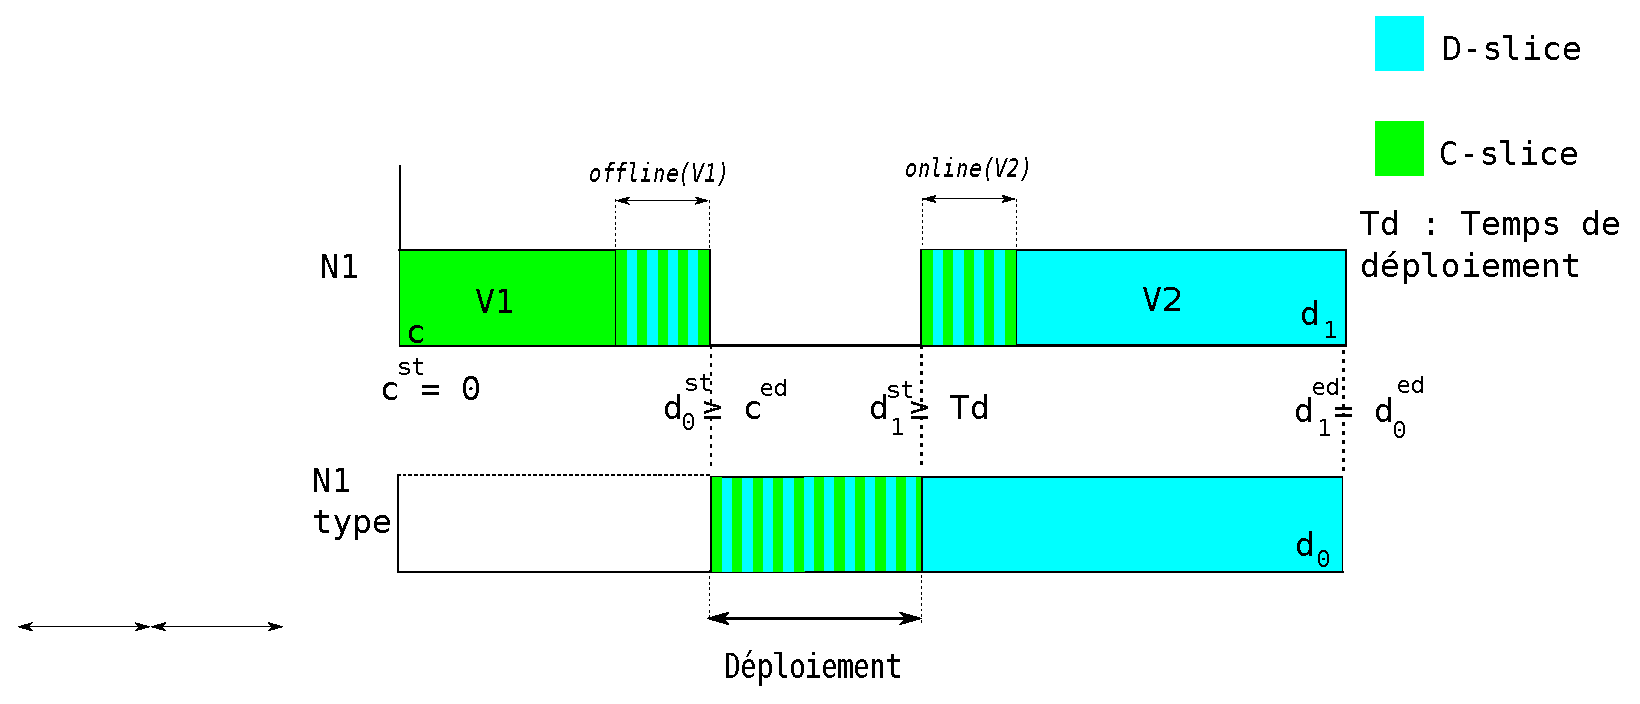
\includegraphics[scale=.45]{imgs/config.eps}
	\caption{\label{config} Exemple de configuration mettant en œuvre un
		changement de type; $v_1$ est mise hors-ligne, $v_2$ est allumée}
\end{figure}

Sur la figure \ref{config}, $v_1$ et $v_2$ sont deux machines
virtuelles de types différents, par exemple Xen et VMWare.
Pour simplifier le problème, on ne considère que des actions
de démarrage et d'éteignage pour les VMs. En effet, on pourrait
remplacer celles-ci par des migrations par exemple, ce qui
nécessiterait de mettre en ligne d'autres nœuds, donc d'augmenter
la complexité de la configuration.

L'opération de déploiement sur le nœud $n_1$ se résume à:
\begin{enumerate}
	\item mettre hors-ligne $v_1$;
	\item éteindre $n_1$;
	\item allumer $n_1$ en changeant son type, c'est-à-dire en changeant
		son hyperviseur.
	\item démarrer $v_2$;
\end{enumerate}
Le temps $T_d$ pris par cette opération est spécifié par l'admninistrateur
du datacenter dans la configuration de BtrPlace.

Pour que la reconfiguration puisse avoir lieu, les contraintes suivantes
doivent être respectées:
\begin{itemize}
	\item Par convention, l'opération de changement de type commence quand
		l'utilisation mémoire de $n_1$ est nulle, ie. lorsqu'aucune VM
		ne tourne dessus;
	\item $d_0^{st} \geq c^{ed}$;
	\item $d_1^{st} \geq T_d$;
\end{itemize}

\subsection{Type connu à l'avance}
Lorsque le nouveau type est une propriété du modèle qui n'a pas à être
déterminée par le solveur, le problème peut être simplifié. L'utilisation
d'une slice pour la dimension de temps devient inutile; on peut se contenter
de deux variables indiquant les temps de début et de fin de l'opération de
déploiement, respectivement notés $D^\mathrm{st}$ et $D^\mathrm{ed}$.

Le type du nœud étant modifié, les VMs présentes au début de la reconfiguration
doivent nécessairement être déplacées ou migrées, suivant les autres
contraintes. Les nouvelles VMs peuvent alors être placées à l'aide de
la contrainte \textit{fence}, d'une façon similaire à ce qui se passe dans
\textit{entropy-fh/src/main/java/entropy/plan/choco/constraint/platform/StaticPlatform.java:40}.

Pour satisfaire le placement sur un nœud $n$, deux contraintes supplémentaires sont
données au solveur:
\begin{enumerate}
	\item Les anciennes VMs partent avant le début de l'opération de
		redéploiement, c'est-à-dire,
\[
	(\forall c \in \mathcal C), P(c) = n \Rightarrow c^\mathrm{ed} \leq D^\mathrm{st}
\]
	\item Les nouvelles VMs arrivent une fois le redéploiement terminé,
		c'est-à-dire:
\[
	(\forall d \in \mathcal D), P(d) = n \Rightarrow d^\mathrm{st} \geq D^\mathrm{ed}
\]
\end{enumerate}

% \subsection{Sans changement de type}
% On observe maintenant ce qu'il se passe si le type reste constant, de
% façon à s'assurer que l'ajout d'une nouvelle dimension ne soit pas
% problématique:
% \begin{figure}[!ht]
% 	\centering
% 	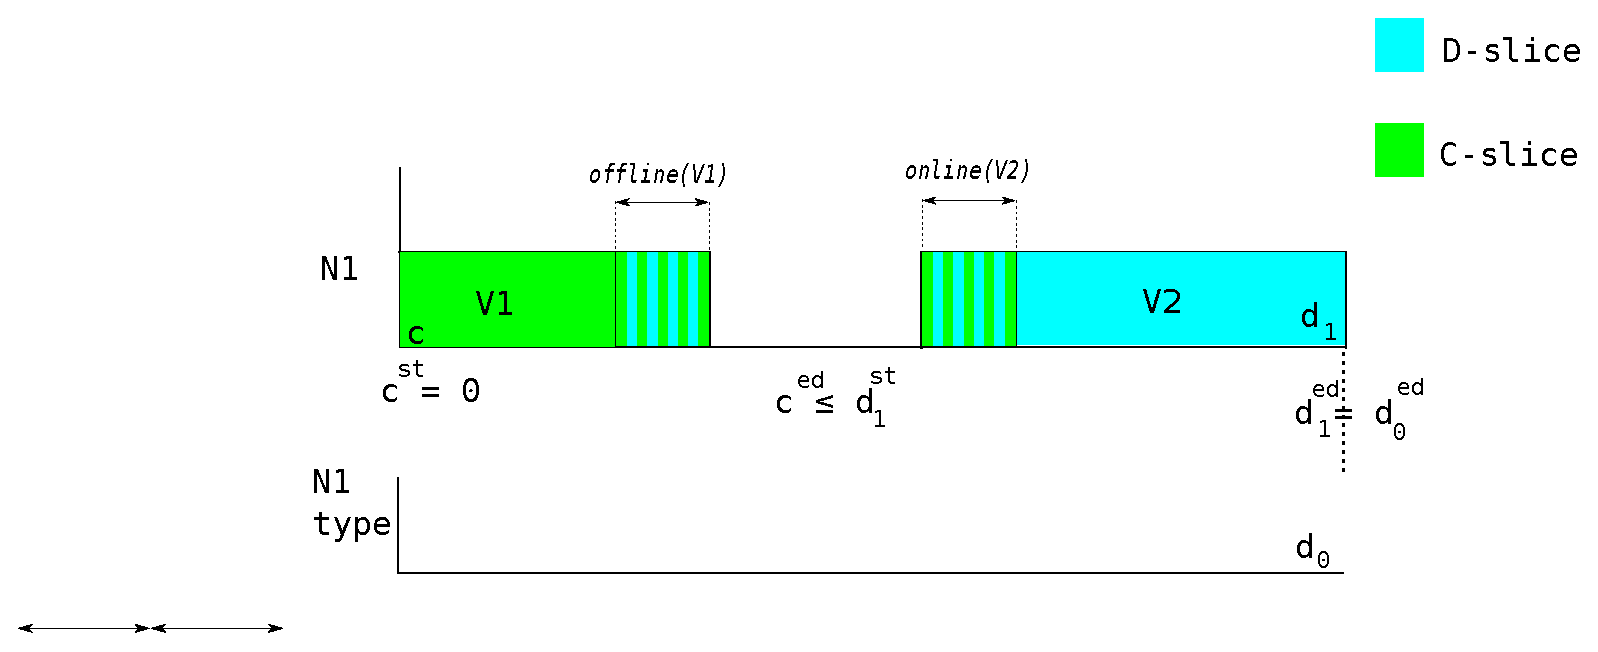
\includegraphics[scale=.45]{imgs/config2.eps}
% 	\caption{\label{config2} Exemple similaire à celui de la figure
% 		\ref{config}, mais sans changement de type, les deux VMs sont
% 		donc du même type; $v_1$ est mise hors-ligne, $v_2$ est allumée}
% \end{figure}

\section{Formalisation}
Le placement est satisfait ssi chaque VM est bien placée sur
un nœud de même type, ie.:
\[
	(\forall v \in \mathcal V), (\exists n \in \mathcal N), P(v) = n
		\Rightarrow T(n) = T(v)	
\]

Cette contrainte doit être implémentée dans BtrPlace via Choco.

\newpage
\selectlanguage{francais}
\bibliographystyle{alpha}
\bibliography{docs}

\end{document}
